% 3blue1brown-inspired geometric visualization of Bayes theorem
% https://youtu.be/HZGCoVF3YvM

\documentclass[tikz]{standalone}

\usetikzlibrary{decorations.pathreplacing}

\begin{document}
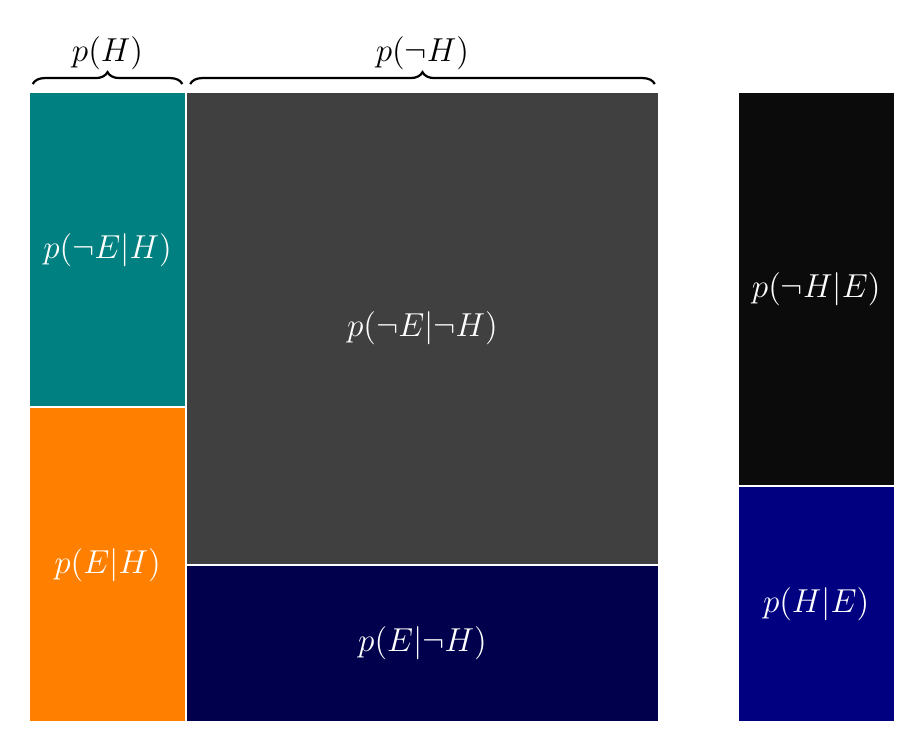
\begin{tikzpicture}[thick, font=\large, white, draw=white]

  \draw[fill=orange] (0,0) rectangle (2,4) node[midway] (pEH) {$p(E|H)$};
  \draw[fill=teal] (0,4) rectangle (2,8) node[midway] (pH) {$p(\neg E|H)$};
  \draw[fill=blue!30!black] (2,0) rectangle (8,2) node[midway] (pH) {$p(E|\neg H)$};
  \draw[fill=gray!50!black] (2,2) rectangle (8,8) node[midway] (pH) {$p(\neg E|\neg H)$};

  \draw[black, decorate, decoration={brace, amplitude=1ex, raise=3pt}] (0.05,8) -- (1.95,8) node[midway, above=1ex] {$p(H)$};
  \draw[black, decorate, decoration={brace, amplitude=1ex, raise=3pt}] (2.05,8) -- (7.95,8) node[midway, above=1ex] {$p(\neg H)$};

  \draw[fill=blue!50!black] (9,0) rectangle (11,3) node[midway] (pH) {$p(H|E)$};
  \draw[fill=gray!9!black] (9,3) rectangle (11,8) node[midway] (pH) {$p(\neg H|E)$};

\end{tikzpicture}
\end{document}
